\newpage
\chapter{Analisis dan Perancangan} \label{Bab III}

\section{Alur Penelitian} \label{III.Alur}
berikut merupakan alur penelitian yang dilakukan oleh peneliti.
\begin{figure}[H]
	\centering
	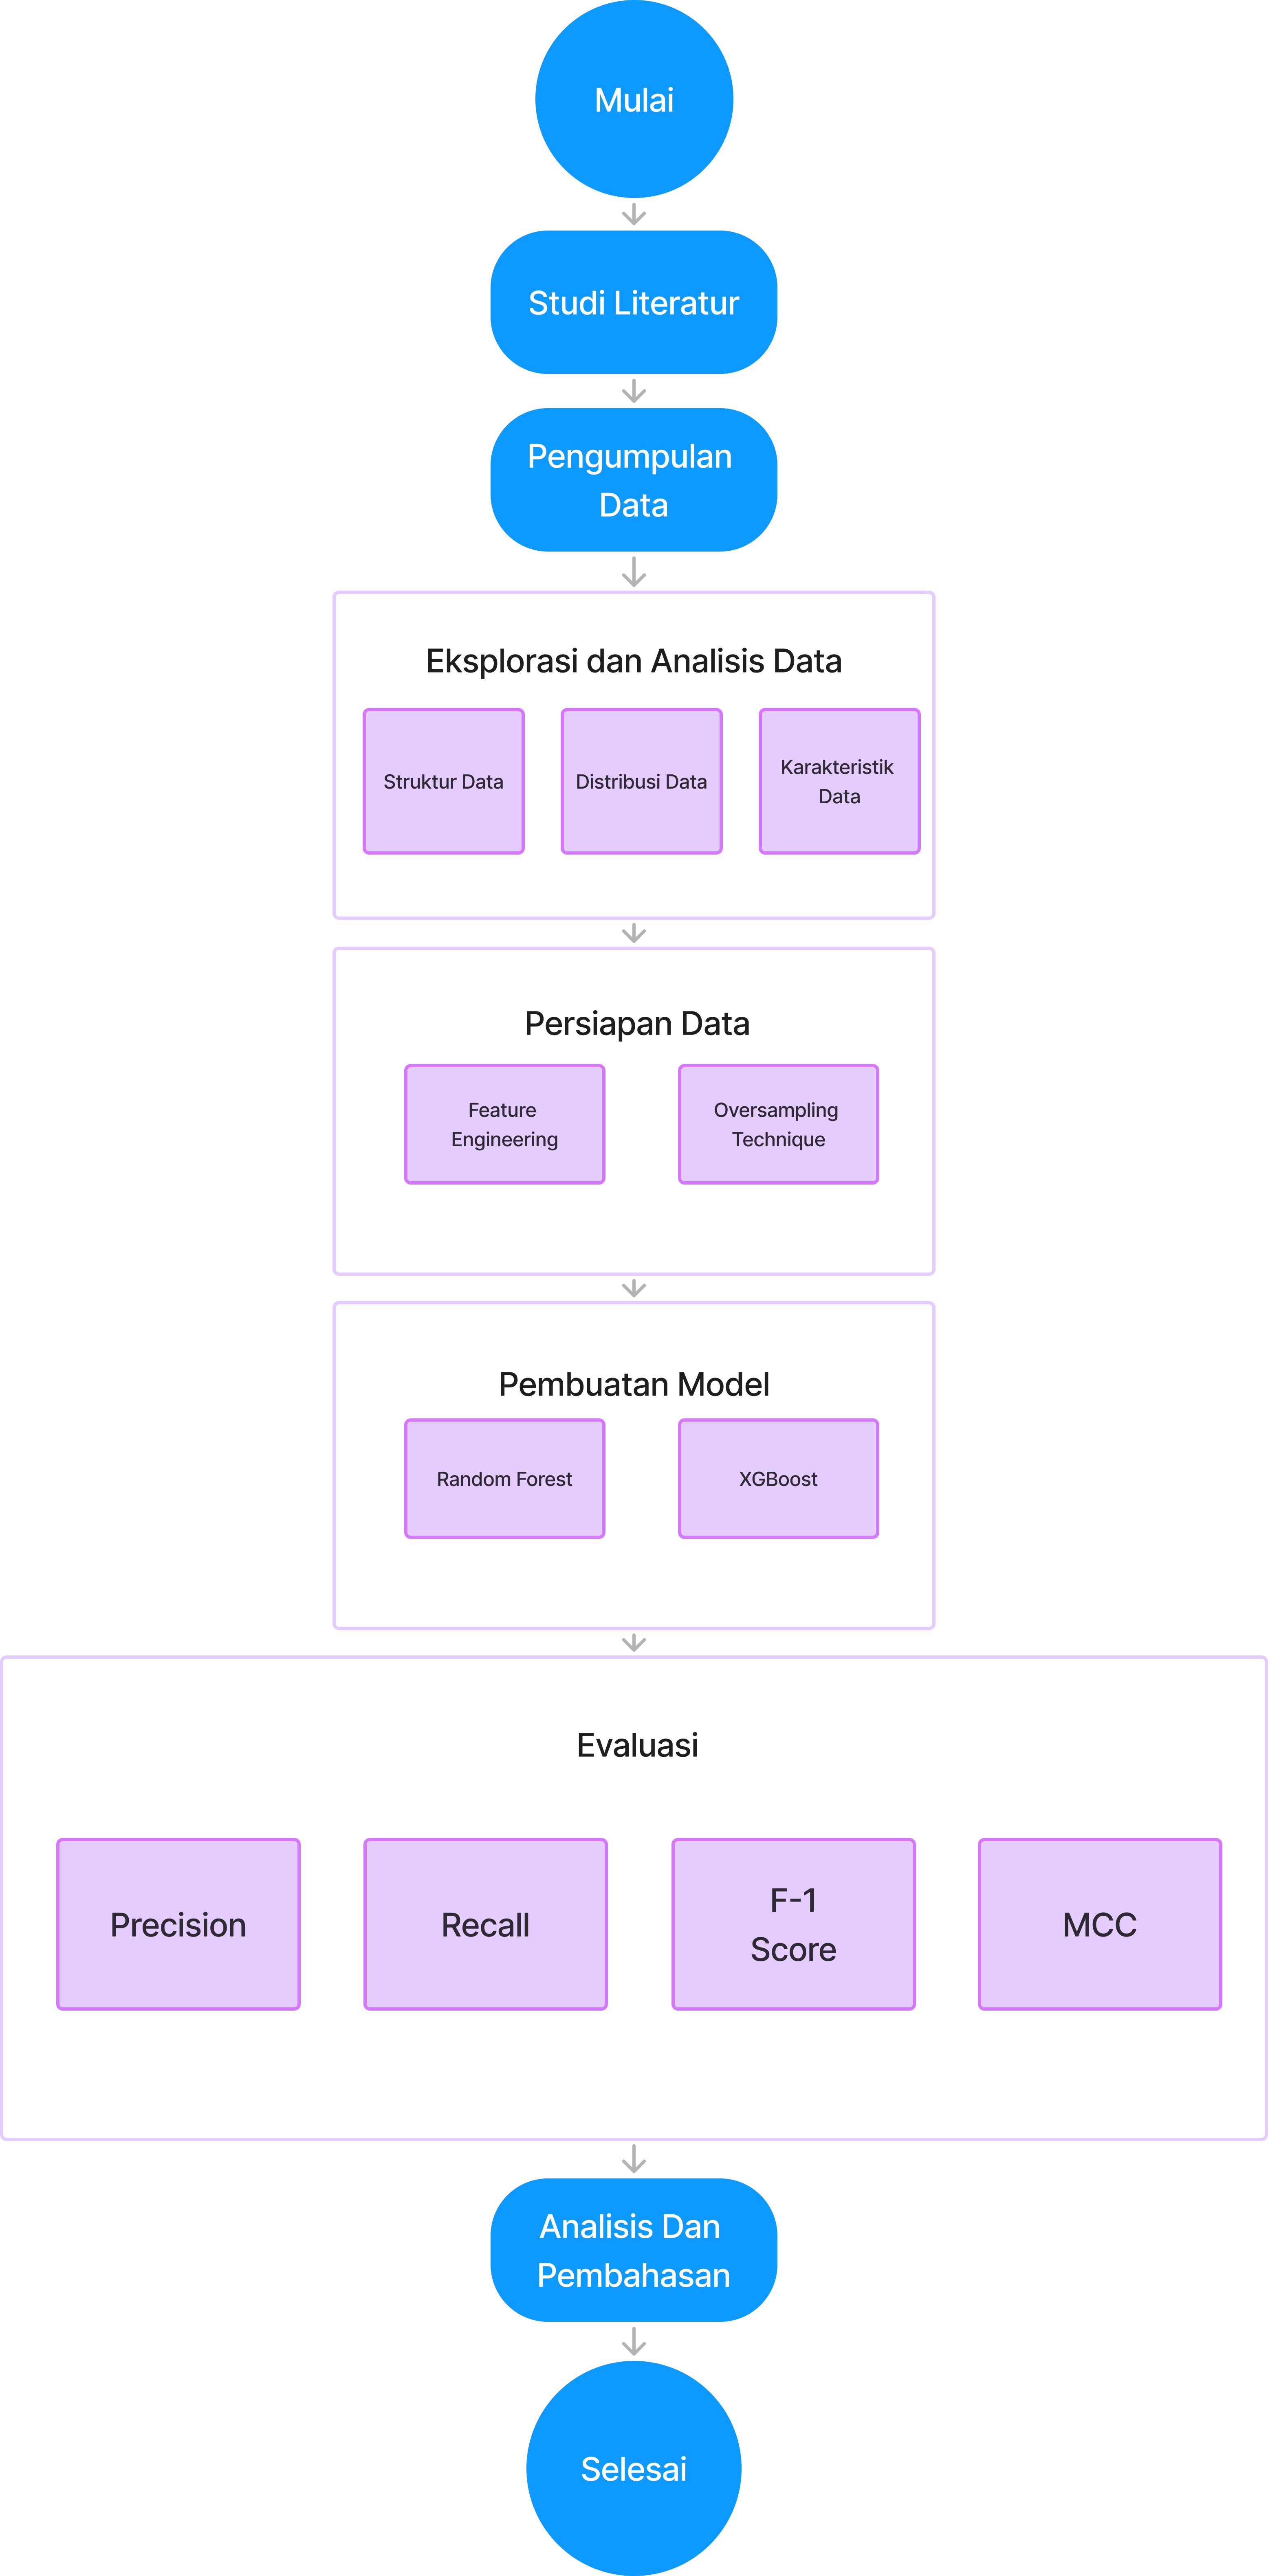
\includegraphics[width=0.5\textwidth]{figure/alur_penelitian.png}
	\caption{Alur Penelitian}
	\label{fig:3.alur penelitian}
\end{figure}

\section{Penjabaran Langkah Penelitian} \label{III.Jabar Alur}
Alur penelitian yang akan dilakukan memiliki beberapa tahapan yang dilakukan secara bertahap dan terdapat sub tahapan pada persiapan data dan juga pembuatan model yang dapat kita lihat pada gambar \ref{fig:3.Skema Pembuatan Model}.
\begin{figure}[H]
	\centering
	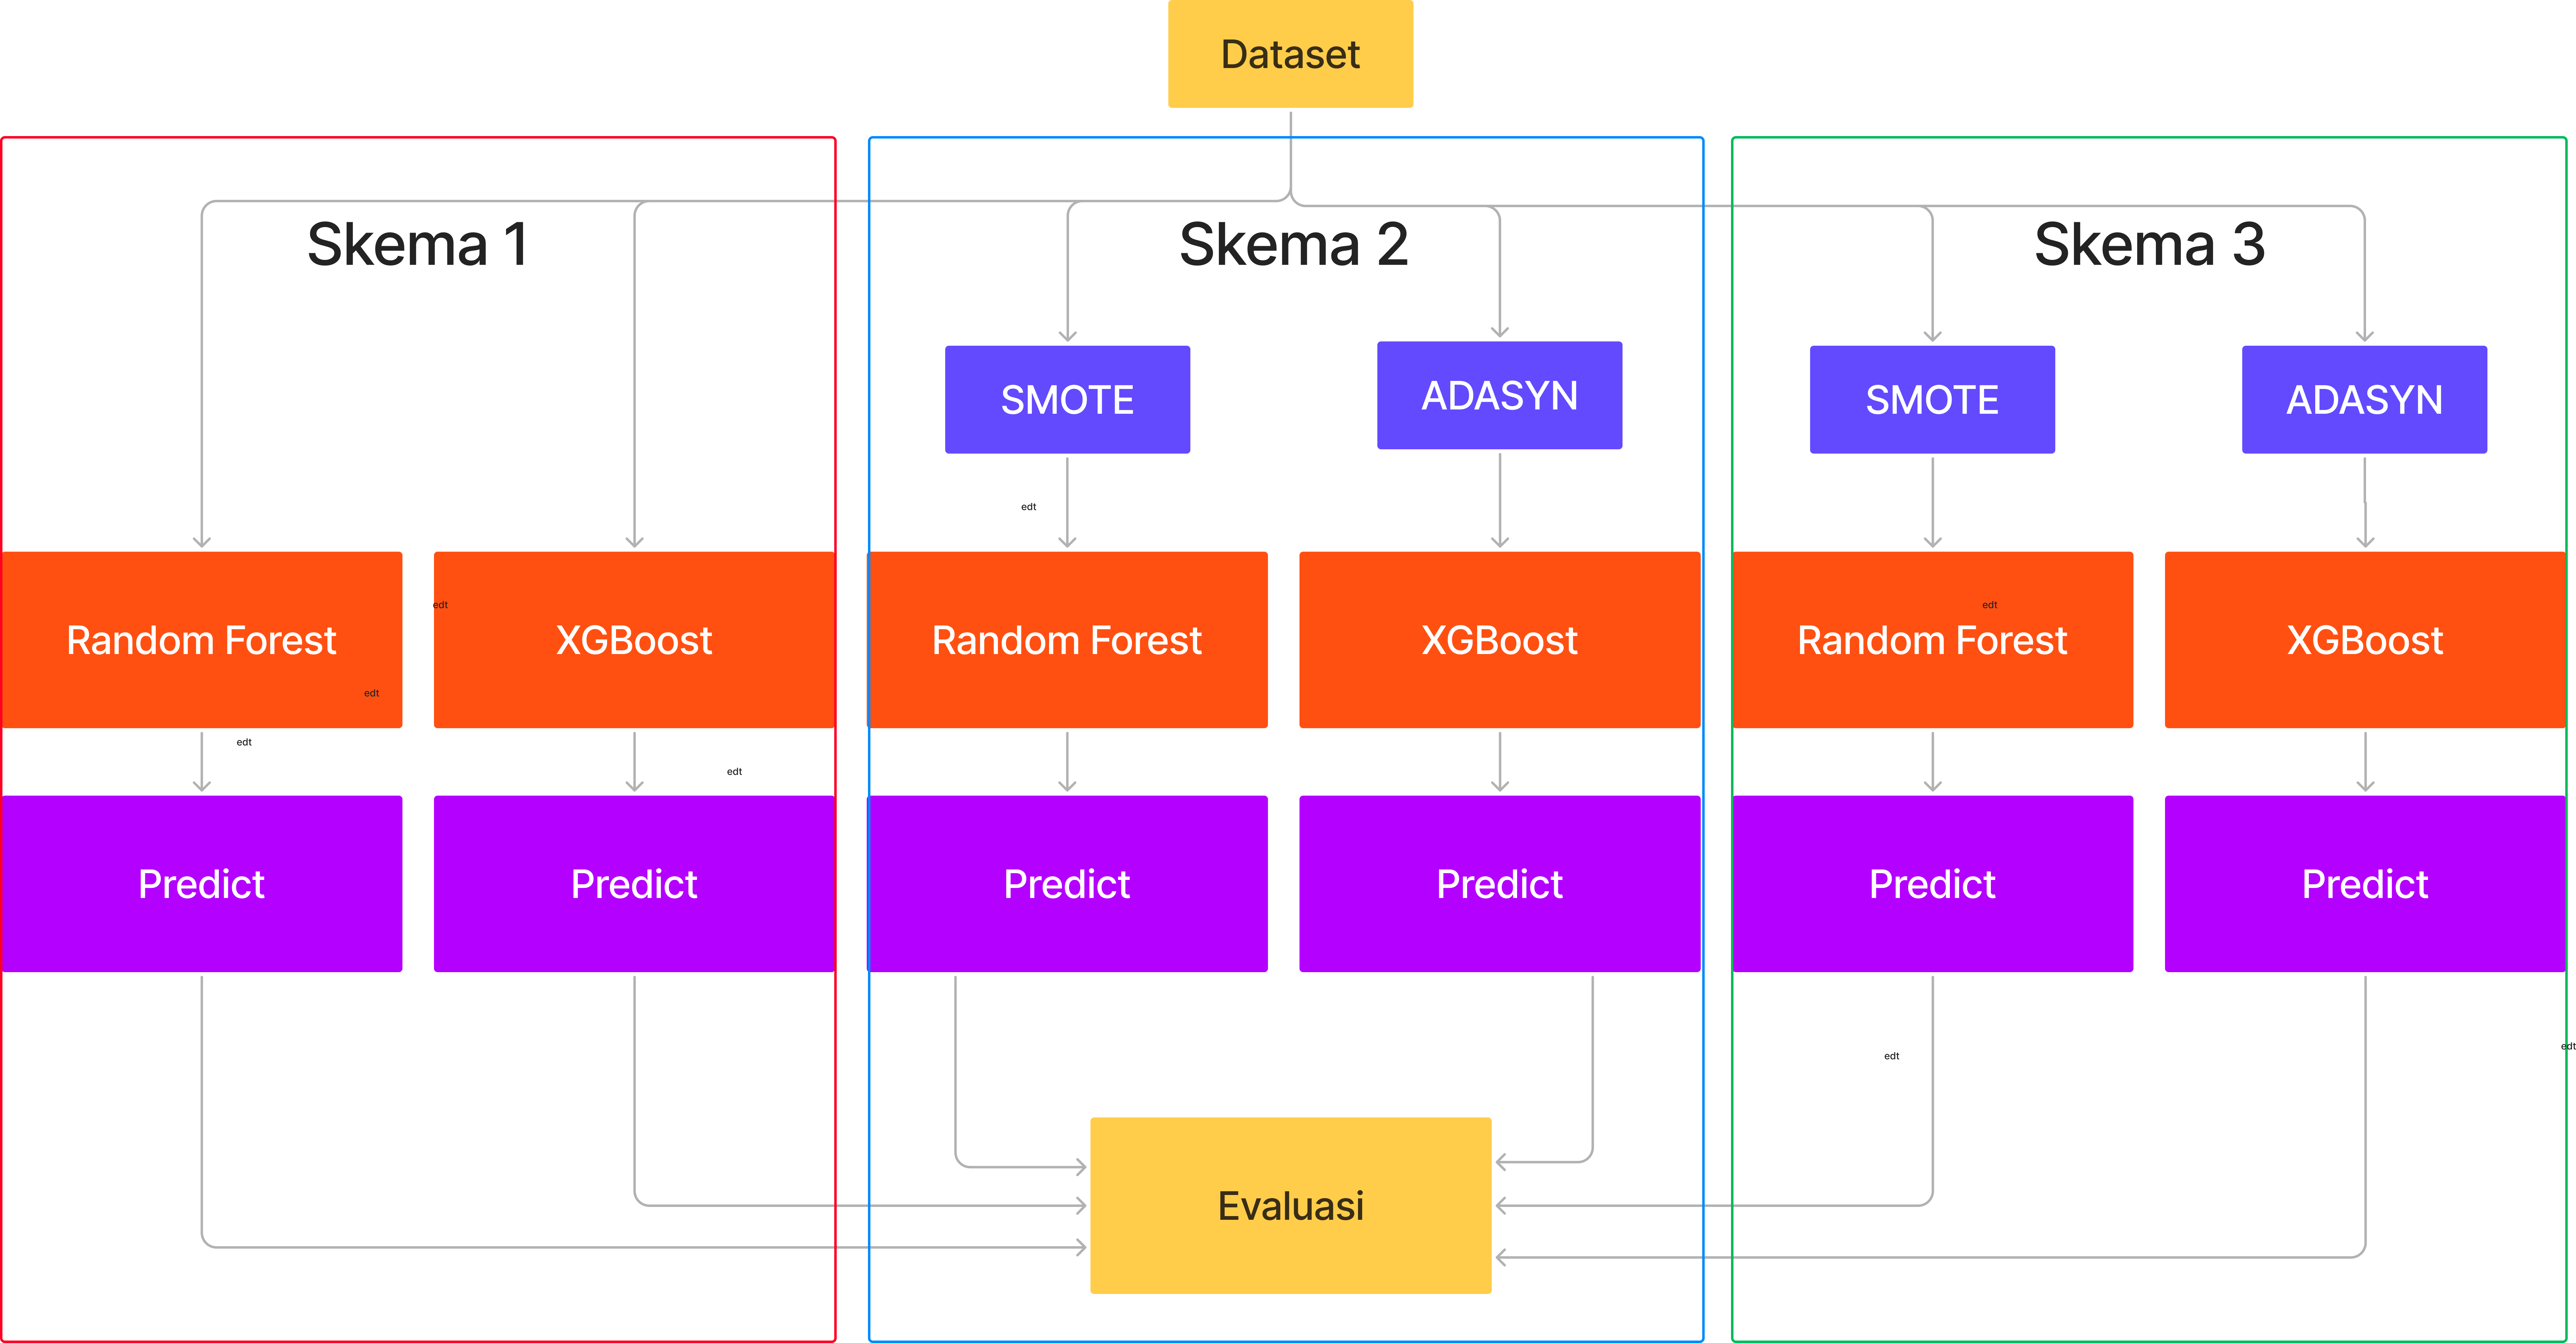
\includegraphics[width=0.7\textwidth]{figure/pembuatanmodel.png}
	\caption{Skema Pembuatan Model}
	\label{fig:3.Skema Pembuatan Model}
\end{figure}

\subsection{Studi Literatur} \label{III.StudiLiteratur}
Proses ini merupakan proses awal yang perlu dilakukan dalam melakukan penilitan guna memahami dan mengetahui teori-teori yang dibutuhkan dalam penelitian. Studi literatur yang dilakukan mencakup algoritma apa yang digunakan dan metode apa yang digunakan dalam membangun model pendeteksi kartu kredit. Hasil dari proses studi literatur yang peneliti lakukan yang berlandasan kepada 6 penelitian yang tinjau pustakanya menunjukan belum adanya analisis yang berfokus kepada teknik oversampling dalam mengatasi transaksi penipuan kartu kredit. Riset-riset sebelumnya banyak berfokus kepada algoritma \textit{machine learning} apa yang digunakan, padahal proses \textit{oversampling} sangat menentukan apakah sebuah algoritma itu bisa berjalan dengan baik atau tidak\cite{ningsih2022analisis}, terkhusus pada kasus deteksi penipuan kartu kredit. \textit{Imbalanced data} pada dataset kartu kredit merupakan hal krusial dalam pembuatan model pendekteksi penipuan kartu kredit dikarenakan dapat membuat model \textit{machine learnng} menjadi bias terhadap kelas minoritas dan salah cara efektif untuk mengatasi masalah hal tersebut ialah dengan menggunakan teknik oversampling\cite{liu2004effect}.
\subsection{Pengumpulan Data} \label{III.pengumpulandata}
Pada proses ini peneliti menggunakan dataset yang dikumpulkan oleh \textit{machine learning group} dari Université Libre de Bruxelles\cite{WinNT,leborgne2022fraud} yang berisi transaksi yang terjadi di eropa. Dataset ini memiliki 492 frauds(penipuan) dari 284.807 transaksi. Dataset ini dipilih oleh peneliti dikarenakan \textit{dataset} tersebut sangat tidak seimbang(\textit{ highly unbalanced}) dengan persentase penipuan sebesar 0.172\% yang dapat dilihat pada gambar \ref{fig:3.Perbandingan Transaksi Normal dan Penipuan} yang membuat dataset tersebut sangat cocok dalam penelitian ini.\\
Dataset tersebut disajikan dalam bentuk file CSV. Dataset tersebut memiliki 30 fitur dan satu label dengan 28 fiturnya sudah dalam bentuk \textit{PCA transformation} guna melindungi privasi data(confidentiality issues) dan 2 fitur lainya tidak dirubah kedalam bentuk PCA adalah \textit{time}, dan \textit{amount} dan untuk label berupa \textit{class}. Fitur 'Time' berisi jumlah detik yang telah berlalu antara setiap transaksi dan transaksi pertama dalam dataset. Fitur 'Amount' merupakan jumlah transaksi. Label 'Class' ini berisi 2 bentuk 1 dan 0 yang mana 1 merupakan \textit{fraud} dan 0 \textit{non-fraud}.
\begin{figure}[H]
	\centering
	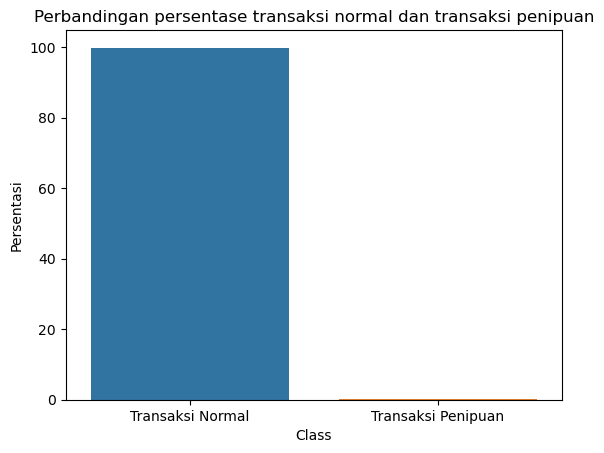
\includegraphics[width=0.5\textwidth]{figure/perbandinganpersentasenormalpenipuan.png}
	\caption{Perbandingan Transaksi Normal dan Penipuan}
	\label{fig:3.Perbandingan Transaksi Normal dan Penipuan}
\end{figure}

\subsection{Eksplorasi dan Analisis Data}
Hasil dari explorasi dan analisis data pada tipe data  dataset \textit{credit card fraud detection} memiliki tipe data \textit{float64} pada hampir semua fiturnya kecuali pada fitur class yang memiliki tipe data \textit{int64} dikarenakan fitur class masih dalam bentuk int64, sebaiknya diubah tipe datanya kedalam bentuk tipe data \textit{category} dikarenakan membuat penggunaan memori menjadi efisien\cite{mckinney2024pandas}. Memori efisien  berpotensi meningkatkan performa dalam \textit{training model}. \\
Peneliti selanjutnya mencoba untuk melakukan analisis dataset pada fitur time dan amount dikarenakan 2 fitur tersebut tidak diubah kedalam bentuk PCA dan peneliti ingin melihat apakah fitur tersebut tetap dipertahankan atau tidak. Pada fitur \textit{time} peneliti akan melakukan observasi distribusi pada transaksi normal dan penipuan berdasarkan waktu dengan menggunakan diagram KDE untuk melihat distribusinya, yang dapat dilihat pada gambar \ref{fig:3.Perbandingan Distribusi Transaksi Normal dan Penipuan Berdasarkan Waktu} yang mana pada figure tersebut bisa kita lihat kalau kedua transaksi normal dan penipuan memiliki distribusi ganda yang memiliki dua puncak yang berarti merupakan \textit{bimodal distribution}\cite{gonick1993cartoon}, hal ini menunjukkan bahwa transaksi dalam dataset terjadi pada dua periode waktu yang berbeda dan setelah itu dapat kita lihat kalau transaksi normal dan penipuan juga merupakan \textit{distribution overlap}\cite{gonick1993cartoon} dikarenakan hal itu kita akan tetap mempertahankan menggunakan \textit{feature} tersebut. 
\begin{figure}[H]
	\centering
	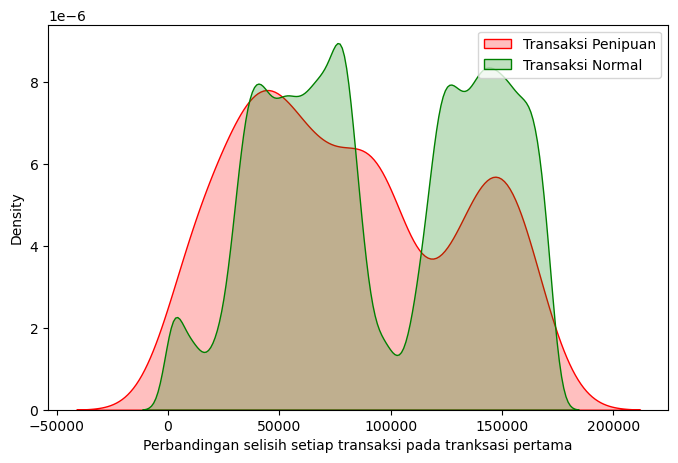
\includegraphics[width=0.5\textwidth]{figure/distribusiwaktunormalpenipuan.png}
	\caption{Perbandingan Distribusi Transaksi Normal dan Penipuan Berdasarkan Waktu}
	\label{fig:3.Perbandingan Distribusi Transaksi Normal dan Penipuan Berdasarkan Waktu}
\end{figure}
Pada fitur \textit{amount} peneliti akan melakukan observasi distribusi pada transaksi normal dan penipuan berdasarkan \textit{amount} yang dilakukan menggunakan diagram KDE sama seperti saat melakukan observasi pada fitur \textit{time}. Berdasarkan hasil observasi distribusi pada gambar \ref{fig:3.Perbandingan Jumlah Transaksi Transaksi Normal dan Penipuan} menunjukan bahwa distribusi dari kedua fitur tersebut merupakan \textit{skewed distribution} yang terpusat pada jumlah transaksi yang rendah(diantara 0 sampai 100) yang dapat kita lihat pada gambar \ref{fig:3.Jumlah Transaksi 0 Sampai 100}. Kedua fitur tersebut merupakan \textit{overlap distribution} namun sedikit perbedaan yang cukup jelas bahwa distribusi transaksi penipuan lebih rendah daripada transaksi normal dan perbedaan selanjutnya pada kedua fitur tersebut ialah transaksi penipuan jarang terjadi pada jumlah transaksi besar(diatas 2500 sampai 25000) yang dapat dilihat pada gambar \ref{fig:3.Jumlah Transaksi 2500 Sampai 25000} dikarenakan banyaknya hubungan yang membedakan transaksi normal dan penipuan, fitur \textit{amount} akan digunakan oleh peneliti.
\begin{figure}[H]
	\centering
	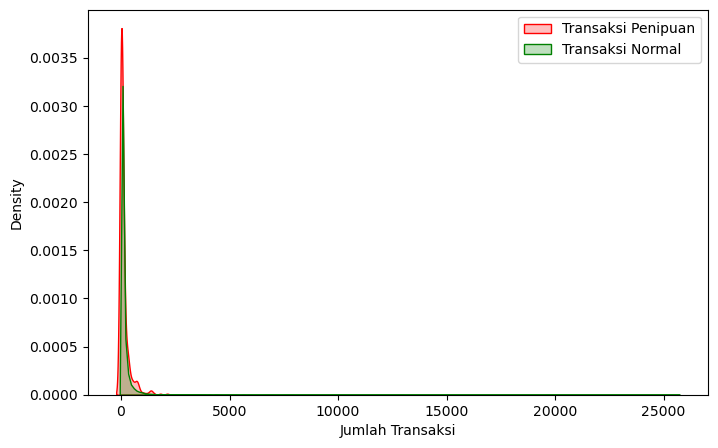
\includegraphics[width=0.5\textwidth]{figure/jumlah transaksi.png}
	\caption{Perbandingan Jumlah Transaksi Transaksi Normal dan Penipuan}
	\label{fig:3.Perbandingan Jumlah Transaksi Transaksi Normal dan Penipuan}
\end{figure}
\begin{figure}[H]
	\centering
	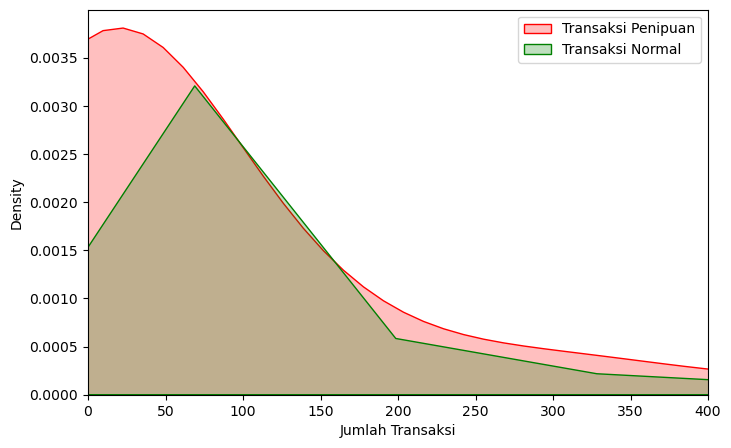
\includegraphics[width=0.5\textwidth]{figure/nolsampaiseratus.png}
	\caption{Jumlah Transaksi 0 Sampai 100}
	\label{fig:3.Jumlah Transaksi 0 Sampai 100}
\end{figure}
\begin{figure}[H]
	\centering
	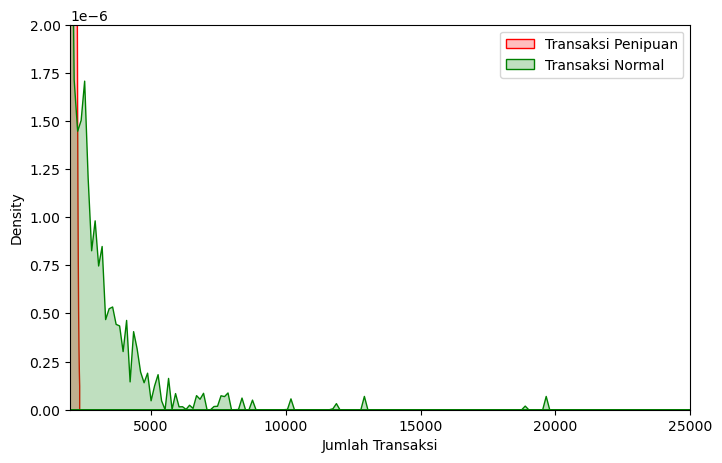
\includegraphics[width=0.5\textwidth]{figure/jumlahtransaksiduaribulimaratus.png}
	\caption{Jumlah Transaksi 2500 Sampai 25000}
	\label{fig:3.Jumlah Transaksi 2500 Sampai 25000}
\end{figure}

\subsection{Persiapan Data}
Proses memuat persiapan data sebelum diinputkan ke dalam \textit{machine learning}. Setelah peneliti melakukan analisis dan eksplorasi data, ada beberapa hal yang perlu dilakukan dalam persiapan data, yang pertama ialah mengecek apakah ada \textit{missing value} didalam dataset, dengan cara mengecek persentase dari setiap feature yang ada pada dataset dengan menggunakan formula berikut:\\

\begin{equation}
       \text{Null\_Percentage}_i = \left( \frac{\sum_{j=1}^{n} \mathbf{1} \{ x_{ij} = \text{null} \}}{n} \right) \times 100
\label{eq:3.missingvalue}
\end{equation}
\myequations{Rumus \textit{missing value}}

Setelah itu peneliti akan melakukan\textit{split} data train dan test dengan metode pengambilan datanya dengan menggunakan \textit{stratified sampling} dengan format 80:20, 80\% data training dan 20\% data test dengan menggunakan modul sklearn model selection dengan melakukan import train\_test\_split. Setelah itu Penelti akan melakukan feature scaling pada feature amount dikarenakan feature amount ukuran nya masih sangat berbeda dibandingkan dengan feature lainya yang sudah dilakukan PCA transformation. Untuk itu, penelti akan melakukan feature scaling dengan menggunakan \textit{Robust Scaling}
dari sklearn. Hasil dari feature scaling pada data training dapat dilihat perubahaannya dari table 3.2 menjadi 3.3.\\
\begin{longtable}{| m{0.6cm} | m{2cm}|}
\caption{5 Data Train Amount Sebelum Scaling} \label{tab:trainingsebelumscaling} \\
\hline
No. & Amount  \\ 
\hline
\endhead
\hline \multicolumn{2}{r}{\textit{Continued}} \\ \hline
\endfoot
\endlastfoot
1 & 7.32  \\ 
\hline
2 & 2.99  \\ 
\hline
3 & 175.10  \\ 
\hline
4 & 6.10  \\ 
\hline
5 & 86.10  \\ 
\hline
\end{longtable}
\begin{longtable}{| m{0.6cm} | m{2cm}|}
\caption{5 Data Train Amount Sesudah Feature Scaling} \label{tab:trainingsesudahscaling} \\
\hline
No. & Amount  \\ 
\hline
\endhead
\hline \multicolumn{2}{r}{\textit{Continued}} \\ \hline
\endfoot
\endlastfoot
1 & 0.000258  \\ 
\hline
2 & 0.000161  \\ 
\hline
3 & 0.006816  \\ 
\hline
4 & 0.000237  \\ 
\hline
5 & 0.003351  \\ 
\hline
\end{longtable}
Selanjutnya peneliti akan melakukan metode \textit{oversampling} yang akan diimplementasikan pada skema 2 dan 3 yang dapat divisualisasikan kedalam plot diagram. namun sebelum itu, agar dapat divisualisasikan kedalam plot diagram yang berupa 2 dimensi data harus diubah dimensinya dikarenakan data yang kita miliki merupakan 30 dimensi, perubahan dimensi tanpa menghilangkan relationship data ialah dengan menggunakan T-SNE dikarenakan T-SNE , hasil dari T-SNE dapat dilihat pada gambar \ref{fig:3.Visualisasi Data TSNE sebelum dan Sesudah SMOTE dan ADASYN}. 
\begin{figure}[H]
	\centering
	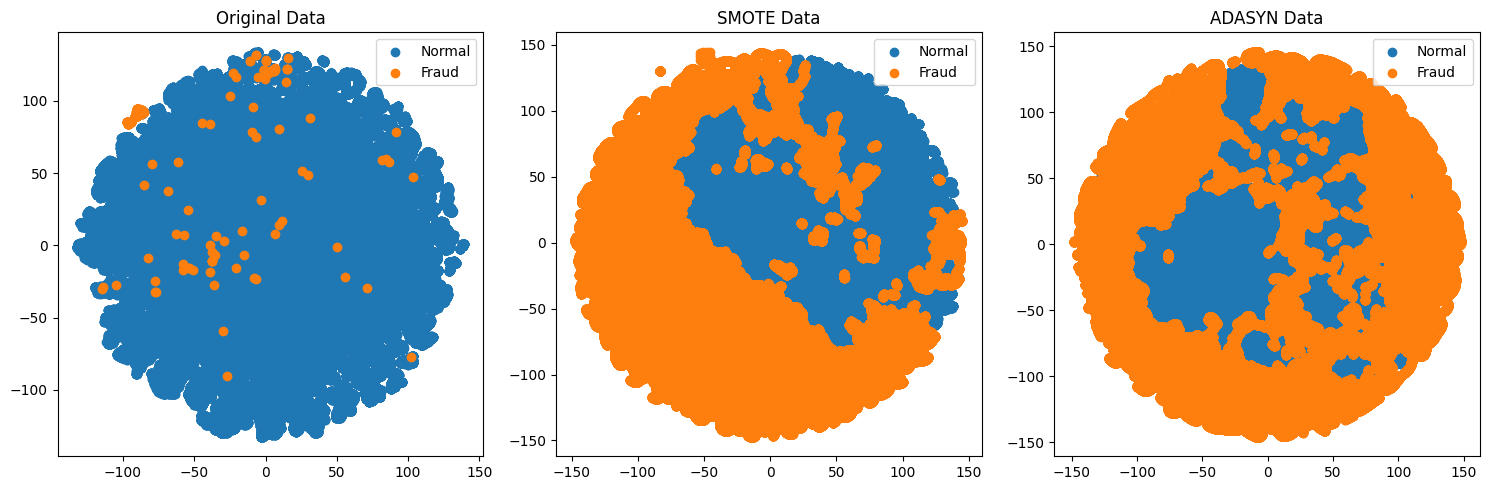
\includegraphics[width=0.7\textwidth]{figure/plot tsne.png}
	\caption{Visualisasi Data TSNE sebelum dan Sesudah SMOTE dan ADASYN}
	\label{fig:3.Visualisasi Data TSNE sebelum dan Sesudah SMOTE dan ADASYN}
\end{figure}

\subsection{Pembuatan Model}
\begin{figure}[H]
	\centering
	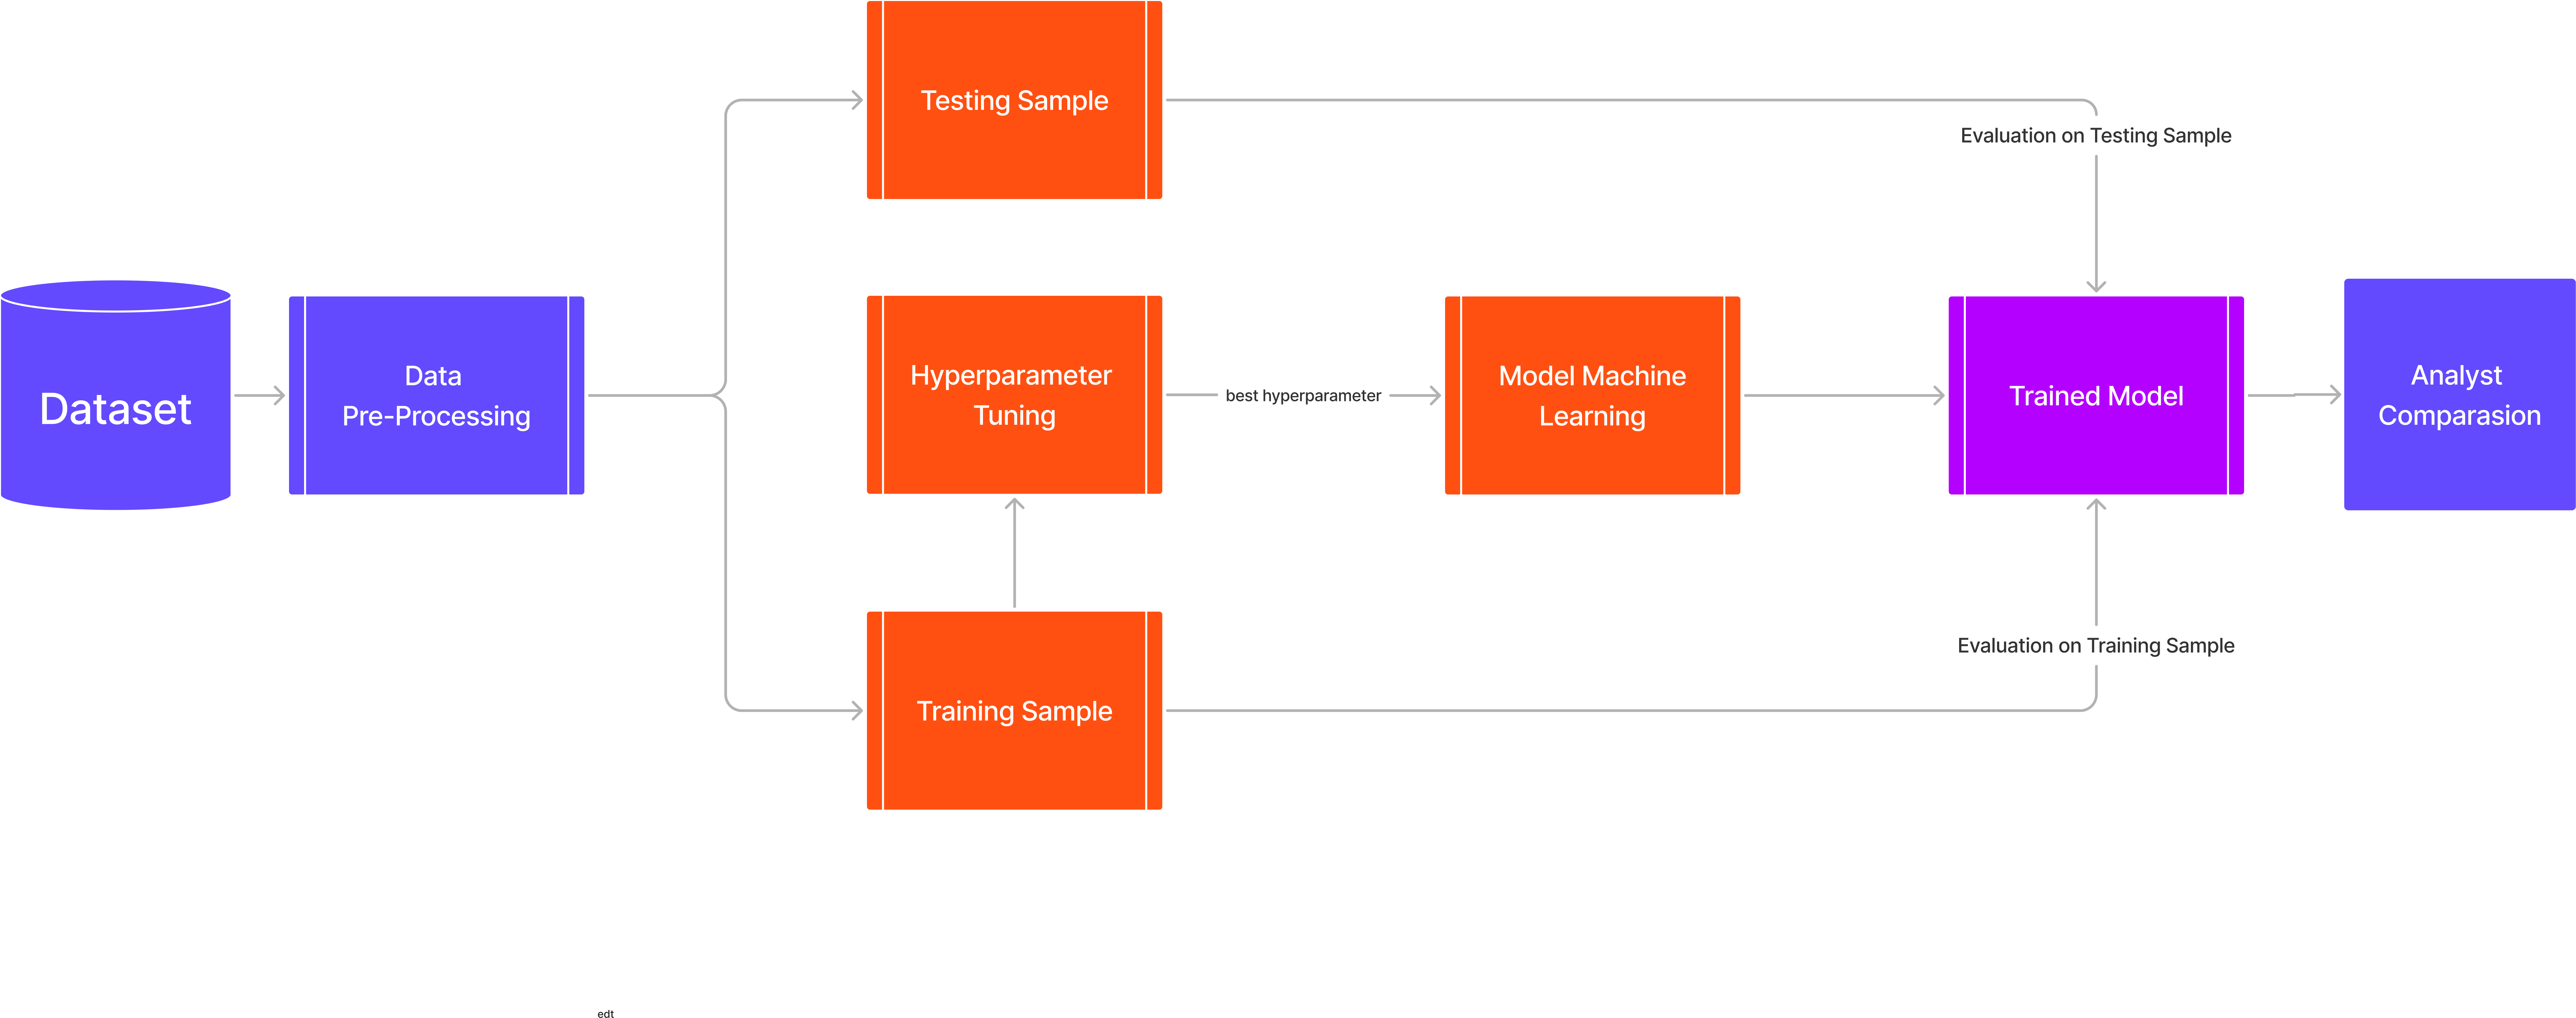
\includegraphics[width=0.7\textwidth]{figure/AlurPembuatanModel.png}
	\caption{Alur Pembuatan Model}
	\label{fig:3.alur pembuatan model}
\end{figure}
Proses ini akan berfokus pada tuning \textit{hyperparameter} model machine learning dengan \textit{cross validation} dengan menggunakan scoring mcc dan melakukan \textit{training model} dengan nilai \textit{hyperparameter} terbaik. Tuning Hyperparameter dilakukan dengan menggunakan \textit{hyperparameter optimization framework} bernama optuna. Pada algoritma \textit{machine learning random forest} \textit{hyperparameter} yang akan dituning berupa\cite{albahli2024efficient}:
\begin{enumerate}[noitemsep]
    \item n\_estimator dengan range nilai dari 200 ke 500.
    \item max\_depth dengan range nilai 5 ke 30.
    \item min\_sample\_split dengan range nilai 5 ke 30.
    \item min\_sample\_leaf dengan range nilai 5 ke 30.
    \item max\_feature dengan pilihan 'auto', 'sqrt', dan 'log2'.
    \item bootstrap dengan pilihan \textit{true} or \textit{false}.
\end{enumerate}
Pada algoritma \textit{machine learning xgboost} \textit{hyperparamter} yang akan dituning dengan menggunakan optuna adalah sebagai berikut\cite{Verma2024ExploringKX}:
\begin{enumerate}[noitemsep]
    \item max\_depth dengan range 3 ke 10.
    \item learning\_rate dengan range 0.01 ke 0.1.
    \item n\_estimator dengan range 200 ke 500.
    \item min\_child\_weight dengan range 3 ke 10.
    \item subsample dengan range 0.6 ke 1.0.
    \item colsample\_bytree dengan range 0.6 ke 1.0.
    \item gamma dengan range 0 ke 1.0.
    \item alpha dengan range 0 ke 5.
\end{enumerate}
Setelah melakukan hyperparameter tuning penelti akan memilih \textit{hyperparameter} terbaik untuk membuat model random forest dan juga xgboost.

\subsection{Evaluasi}
Pengujian dilakukan dengan melihat berdasarkan nilai dari  \textit{precision}, \textit{recall}, \textit{f-1 score}, dan \textit{Matthews’s correlation coefficient} (MCC) pada setiap model yang digunakan dalam penelitian ini seperti \textit{random forest} dan \textit{xgboost}. Evalusi akan dilakukan dengan 4 skenario yaitu dengan membandingkan  hasil skenario tersebut dan setiap skenario akan membuat dua model \textit{random forest} dan \textit{xgboost} dengan metode tertentu.
\begin{enumerate}[noitemsep]
    \item Skenario pertama: Pada skenario pertama peneliti akan melakukan pengecekan performa dari model \textit{random forest} dan \textit{xgboost} tanpa melakukan metode oversampling, yang artinya model dibuat berdasarkan data yang tidak seimbang. Pengecekan perfoma akan dilihat berdasarkan \textit{precision}, \textit{recall},     \textit{f1-score}, dan \textit{Matthews’s correlation coefficient} (MCC) .
    \item Skenario kedua: pada skenario kedua peneliti akan melakukan pengecekan performa dari model \textit{random forest} dan \textit{xgboost} dengan menggunakan metode oversampling SMOTE. Pengecekan perfoma akan dilihat berdasarkan \textit{precision}, \textit{recall},    \textit{f1-score}, dan \textit{Matthews’s correlation coefficient} (MCC).
    \item Skenario ketiga: pada skenario ketiga peneliti akan melakukan pengecekan performa dari model \textit{random forest} dan \textit{xgboost} dengan menggunakan metode oversampling ADASYN. Pengecekan perfoma akan dilihat berdasarkan \textit{precision}, \textit{recall}, \textit{f1-score}, dan \textit{Matthews’s correlation coefficient} (MCC).
    \item Skenario keempat: pada skenario keempat peneliti akan melakukan pengecekan performa secara menyeluruh dengan membandingkan seluruh hasil dari setiap 6 percobaan yang dilakukan dan menentukan hasil percobaan terbaik dengan melihat metriks performa berdasarkan \textit{precision}, \textit{recall}, \textit{f1-score}, dan \textit{Matthews’s correlation coefficient} (MCC).
\end{enumerate}
\subsection{Analisis dan Pembahasan}
Pada tahap in, dilakukan analisis lebih lanjut beserta pembahasan secara detail terhadap pengujian yang telah dilakukan. Setelah melakukan analisis akan dilakukan proses pembahasan dalam bentuk penulisan laporan.


\subsection{Perhitungan SMOTE}
Perhitungan SMOTE dimulai dengan mengetahui data minoritas, sebagai contoh kita memiliki 3 data minortas yaitu:
\begin{enumerate}
	\item Sample A: (2, 3)
	\item Sample B: (4, 7)
	\item Sample C: (3, 4)
\end{enumerate}
Setelah mengetahui data minoritas kita akan mencari \textit{iniitial sample} yang didapatkan dengan melakukan pemilihan acak. Setelah itu, kita akan mencari tetangga terdekat dari \textit{initial sample} ke sampel lainnya dengan menggunakan \textit{Euclidean distance}. Untuk mendapatkan nilai \textit{Euclidean distance} itu dengan menggunakan teorema pythagoras dengan rumus:\\
 \begin{equation}
	 d = \sqrt{(x_2 - x_1)^2 + (y_2 - y_1)^2}
\end{equation}
\label{eq:3.teorema pythagoras}
\\
\myequations{Rumus Teorema Pythagoras}
Kita dapatkan secara acak \textit{intial sample} yaitu sampel A dan selanjutnya kita akan menghitung \textit{Euclidean distance}.
\begin{enumerate}
	\item  Jarak A ke B.\\
		$$
			d_{AB} = \sqrt{(4-2)^2 + (7-3)^2} = \sqrt{2^2 + 4^2} = \sqrt{4 + 16} = \sqrt{20} \approx 4.47
		$$

	\item Jarak A ke C.\\
		$$
			d_{AC} = \sqrt{(3-2)^2 + (4-3)^2} = \sqrt{1^2 + 1^2} = \sqrt{1 + 1} = \sqrt{2} \approx 1.41
		$$
\end{enumerate}
Karena $d_{AC} < d_{AB}$, sampel C merupakan tetangga terdekat dari sampel A. Setelah mengetahui tetangga terdekat, selanjutnya, kita akan membuat data sintetis dengan menggunakan rumus 2.\ref{eq:2.smote}.
\begin{itemize}
	\item Sampel A: (2,3).
	\item Sample C (tetangga terdekat): (3,4).
	\item $\lambda: 0.5$ (dipilih secara acak)
\end{itemize}
Menghitung perbedaan sampel A dan sampel C:
\\
\begin{align*}
    x_{synthetic} &= \text{Sampel A} + \lambda \cdot (\text{Sampel C} - \text{Sampel A})   \\
    x_{synthetic} &= \text{Sampel A} + \lambda \cdot ((3-2), (4-3)) \\
    x_{synthetic} &= \text{Sampel A} + \lambda \cdot (1,1) 
\end{align*}
\\
Mengkalikan dengan lamdha:
\\
\begin{align*}
    x_{synthetic} &= \text{Sampel A} + 0.5 \cdot (1,1) \\ 
    x_{synthetic} &= \text{Sampel A} + (0.5,0.5) 
\end{align*}
\\
Menghasilkan data sintetis:
\\
\begin{align*}
    x_{synthetic} &= (2,3) + (0.5,0.5) \\
    x_{synthetic} &= (2.5, 3.5) 
\end{align*}
\\
data sintetis yang telah berhasil dibuat adalah (2.5, 3.5).
 
\subsection{Perhitungan ADASYN}
Perhitungan ADASYN dimulai dengan mengetahui data mayoritas dan data minoritas. Kita asumsikan kita memliki dataset seperti berikut:
\begin{itemize}
	\item Sampel Minoritas.
		\begin{enumerate}
			\item Sampel A: (2,3).
			\item Sampel B: (3,7).
		\end{enumerate}
	\item Sampel Majoritas.
		\begin{enumerate}
			\item Sampel M1: (2.5, 3.2).
			\item Sampel M2: (2.7, 3.1).
			\item Sample M3: (6,9).
		\end{enumerate}
\end{itemize}
Dan kita akan menginisiasi nilai k(\textit{number of nearest neighbors} = 3 dan total data sintetis yang ingin kita buat adalah 9 $(G = 9)$. Setelah itu kita akan mencari tetangga terdekat dari setiap data minoritas dengan rumus 3.\ref{eq:3.teorema pythagoras}.
Untuk data minortas pada sampel A(2, 3):
\begin{enumerate}
	\item  Jarak A ke M1.\\
		$$
			d_{AM1} = \sqrt{(2.5-2)^2 + (3.2-3)^2} = \sqrt{0.5^2 + 0.2^2} = \sqrt{0.25 + 0.04} = \sqrt{0.29} \approx 0.54
		$$

	\item Jarak A ke M2.\\
		$$
			d_{AM2} = \sqrt{(2.7-2)^2 + (3.1-3)^2} = \sqrt{0.7^2 + 0.1^2} = \sqrt{0.49 + 0.01} = \sqrt{0.50} \approx 0.71 
		$$

	\item Jarak A ke M3.\\
		$$
			d_{AM3} = \sqrt{(6-2)^2 + (9-3)^2} = \sqrt{4^2 + 6^2} = \sqrt{16 + 36} = \sqrt{52} \approx 7.21 
		$$
		
	\item Jarak A ke B.\\
		$$
			d_{AB} = \sqrt{(4-2)^2 + (7-3)^2} = \sqrt{2^2 + 4^2} = \sqrt{4 + 16} = \sqrt{20} \approx 4.47 
		$$
\end{enumerate}
Pada sampel A 3 tetangga terdekat A$(k = 3)$ ialah M1,M2, dan B. yang berarti ratio dari sampel A adalah:

$$
r_A = \frac{Majority}{k} = \frac{2}{3} \approx 0.67
$$
\\
Untuk data minoritas pada sampel B(4, 7):
\begin{enumerate}
	\item  Jarak B ke M1.\\
		$$
			d_{BM1} = \sqrt{(4-2.5)^2 + (7-3.2)^2} = \sqrt{1.5^2 + 3.8^2} = \sqrt{2.25 + 14.44} = \sqrt{16.69} \approx 4.09
		$$

	\item Jarak B ke M2.\\
		$$
		d_{BM2} = \sqrt{(4-2.7)^2 + (7-3)^2} = \sqrt{1.3^2 + 3.9^2} = \sqrt{1.69 + 15.21} = \sqrt{16.9} \approx 4.11 
		$$

	\item Jarak B ke M3.\\
		$$
			d_{BM3} = \sqrt{(4-6)^2 + (7-9)^2} = \sqrt{(-2)^2 + (-2)^2} = \sqrt{4 + 4} = \sqrt{16} \approx 2.83 
		$$
		
	\item Jarak A ke B.\\
		$$
			d_{BA}  \approx 4.47 
		$$
\end{enumerate}
Pada sampel B 3 tetangga terdekat $(k = 3)$ ialah M3,M1, dan M2. yang berarti ratio dari sampel B adalah:

$$
r_B = \frac{Majority}{k} = \frac{3}{3} = 1 
$$
\\
Menentukan alokasi data sintetis:\\
$$
R_total = r_a + r_b = 0.69 + 1 = 1.69
$$
\\
Menghitung \textit{weight} pada setiap minority sampel:

\begin{itemize}
	\item \textit{weight} dari sampel A: \\ 
		$$
			w_A = \frac{r_a}{R_total} = \frac{0.67}{1.67} \approx 0.40
		$$
	\item \textit{weight} dari sampel B:\\
		$$
			w_B = \frac{r_b}{R_total} = \frac{1}{1.67} \approx 0.60
		$$
\end{itemize}

Maka jumlah data sintetis pada masing data minoritas ialah:
\begin{itemize}
	\item Data sintetis pada sampel A:\\
		$$
			G_A = w_A \times G \approx 0.40 \times 9 \approx 3.6 
		$$
	\item Data sintetis pada sample B:\\
		$$
			G_B = w_B \times G \approx 0.60 \times 9 \approx 5.4 
		$$
\end{itemize}
Jumlah dari masing-masing data sintetis ialah 4(dibulatkan) pada sampel A dan 5(dibulatkan) pada sampel B. Setelah mengalokasikan berapa data sintetis yang akan dibuat, dilanjutkan dengan membuat data sintetis pada setiap data minoritas dengan menggunakan rumus 2.\ref{eq:2.smote}. Kita asumsikan bahwa kita memilih secara acak data minoritas dan yang terpilih ialah sampel A dan tetangga terdekat yang terpilih ialah sampel B(karena sampel B merupakan satu-satunya data minoritas lainnya).\\
Menghitung nilai pembeda dari sampel A dan B:\\
\\
\begin{align*}
    x_{synthetic} &= \text{Sampel A} + \lambda \cdot (\text{Sampel B} - \text{Sampel A})   \\
    x_{synthetic} &= \text{Sampel A} + \lambda \cdot ((4-2), (7-3)) \\
    x_{synthetic} &= \text{Sampel A} + \lambda \cdot (2,4) 
\end{align*}
\\
Mengkalikan dengan lamdha $(\lambda = 0.5)$:
\\
\begin{align*}
    x_{synthetic} &= \text{Sampel A} + 0.5 \cdot (2,4) \\ 
    x_{synthetic} &= \text{Sampel A} + (1,2) 
\end{align*}
\\
Menghasilkan data sintetis:
\\
\begin{align*}
    x_{synthetic} &= (2,3) + (1,2) \\
    x_{synthetic} &= (3, 5) 
\end{align*}
\\
data sintetis yang telah berhasil dibuat adalah (3, 5).
 



\subsection{Alat dan Bahan Tugas Akhir}
Adapun alat dan bahan yang digunakan dalam penelitian ini adalah sebagai berikut:
\subsubsection{Alat}
Berikut adalah alat yang digunakan dalam penelitian ini:
\begin{enumerate}
    \item Spesifikasi Laptop, komputer atau notebook:
    \begin{enumerate}
        \item Minimum spesifikasi komputer, laptop, atau notebook agar dapat melakukan penelitian ini, sebagai berikut:
        \begin{enumerate}
            \item Sistem operasi linux atau  Windows 10 (64-bit), x86-64 based Menggunakan Processor Intel Core i5.
            \item Menggunakan Processor Intel Core i5 atau AMD Ryzen 5.
            \item Kebutuhan RAM paling minimal 8 GB.
            \item Memiliki ruang memori yang bebas setidaknya 10 GB.
        \end{enumerate}
        \item Pada penelitian ini penulis menggunakan laptop dengan spesifikasi sebagai berikut:
        \begin{enumerate}
            \item ubuntu 22.04.4(64-bit),x86\_64 based
            \item AMD Ryzen 5 4600H with Radeon G 
            \item RAM 8.
            \item SSD 512GB
            \item GPU: NVIDIA GeForce GTX 1650 Ti
        \end{enumerate}
    \end{enumerate}
    \item Visual Studio Code
    \item Scikit-Learn
\end{enumerate}
\subsubsection{Bahan}
Berikut adalah bahan yang digunakan dalam penelitian ini:
\begin{enumerate}
    \item Dataset yang digunakan ialah dataset Credit Card Fraud Detection yang dikumpulkan dan dianalisis oleh \textit{machine learning group} Université Libre de Bruxelles(ULB)
    \item Jurnal penelitian   dari penelitian sebelumnya yang dijadikan dasar teori dan rangkaian konsep serta ide untuk mendukung penelitian.
\end{enumerate}


